% Chapter 8: Sprint 5 - Excel Report Generation & System Optimization

\chapter{Sprint 5: Excel Report Generation and System Optimization}

\section{Introduction}

Sprint 5, the final development sprint, implements advanced reporting capabilities and system optimization. This sprint delivers comprehensive Excel report generation enabling stakeholders to analyze intervention data, create organizational archives, and perform metrics analysis. System optimization ensures scalability, performance, and reliability in production environments.

The sprint focuses on business analytics and operational intelligence, providing management with tools to monitor operations, identify trends, and make data-driven decisions. Performance optimization ensures the system can handle growing data volumes and concurrent user load effectively.

\section{Sprint Preview and Objectives}

\subsection{User Stories}

\begin{enumerate}
\item \textbf{US-S5-001: Excel Report Generation}
  \begin{itemize}
  \item \textbf{As a} coordinator
  \item \textbf{I want} to generate comprehensive Excel reports from intervention data
  \item \textbf{So that} I can analyze and share intervention metrics
  \item \textbf{Story Points:} 13
  \end{itemize}

\item \textbf{US-S5-002: Dynamic Report Templates}
  \begin{itemize}
  \item \textbf{As a} manager
  \item \textbf{I want} to configure custom Excel templates for reports
  \item \textbf{So that} reports match organizational standards
  \item \textbf{Story Points:} 8
  \end{itemize}

\item \textbf{US-S5-003: Archive Management}
  \begin{itemize}
  \item \textbf{As a} system
  \item \textbf{I want} to automatically archive old interventions
  \item \textbf{So that} database remains performant
  \item \textbf{Story Points:} 8
  \end{itemize}

\item \textbf{US-S5-004: Performance Optimization}
  \begin{itemize}
  \item \textbf{As a} system
  \item \textbf{I want} to optimize queries and caching
  \item \textbf{So that} system handles large datasets efficiently
  \item \textbf{Story Points:} 8
  \end{itemize}

\item \textbf{US-S5-005: System Monitoring}
  \begin{itemize}
  \item \textbf{As a} administrator
  \item \textbf{I want} to monitor system health and metrics
  \item \textbf{So that} I can identify and resolve issues proactively
  \item \textbf{Story Points:} 8
  \end{itemize}
\end{enumerate}

\subsection{Sprint Goals}

\begin{enumerate}
\item \textbf{Reporting:} Implement comprehensive Excel report generation
\item \textbf{Configuration:} Enable customizable report templates
\item \textbf{Archive:} Implement intelligent data archival strategy
\item \textbf{Performance:} Optimize system for scalability
\item \textbf{Monitoring:} Provide system health visibility
\end{enumerate}

\section{Sprint Backlog}

The 45-point sprint focuses on advanced features and optimization:

\begin{table}[H]
\centering
\caption{Sprint 5 Backlog}
\label{tab:sprint5_backlog}
\begin{tabularx}{\textwidth}{|l|X|l|l|}
\hline
\textbf{ID} & \textbf{User Story} & \textbf{Points} & \textbf{Status} \\
\hline
S5-1 & Excel report generation & 13 & Completed \\
\hline
S5-2 & Dynamic report templates & 8 & Completed \\
\hline
S5-3 & Archive management & 8 & Completed \\
\hline
S5-4 & Performance optimization & 8 & Completed \\
\hline
S5-5 & System monitoring & 8 & Completed \\
\hline
\textbf{Total} & & \textbf{45} & \\
\hline
\end{tabularx}
\end{table}

\section{Functional Specification}

\subsection{Report Generation Process}

The Excel report generation process involves:

\begin{enumerate}
\item \textbf{Data Collection:} Query interventions based on filters
\item \textbf{Template Loading:} Retrieve active report template configuration
\item \textbf{Dynamic Population:} Insert data into Excel using Apache POI
\item \textbf{Calculation:} Compute metrics and aggregations
\item \textbf{Styling:} Apply formatting and themes
\item \textbf{Export:} Generate and download Excel file
\end{enumerate}

\subsection{Report Types}

\begin{itemize}
\item \textbf{Daily Summary:} Interventions completed by day with metrics
\item \textbf{Technician Report:} Performance by technician
\item \textbf{Regional Report:} Geographic analysis of work
\item \textbf{Custom Report:} User-defined filters and metrics
\end{itemize}

\section{Conception}

\subsection{Class Diagram}

\begin{figure}[H]
\centering
\fbox{\parbox{1\textwidth}{
\centering
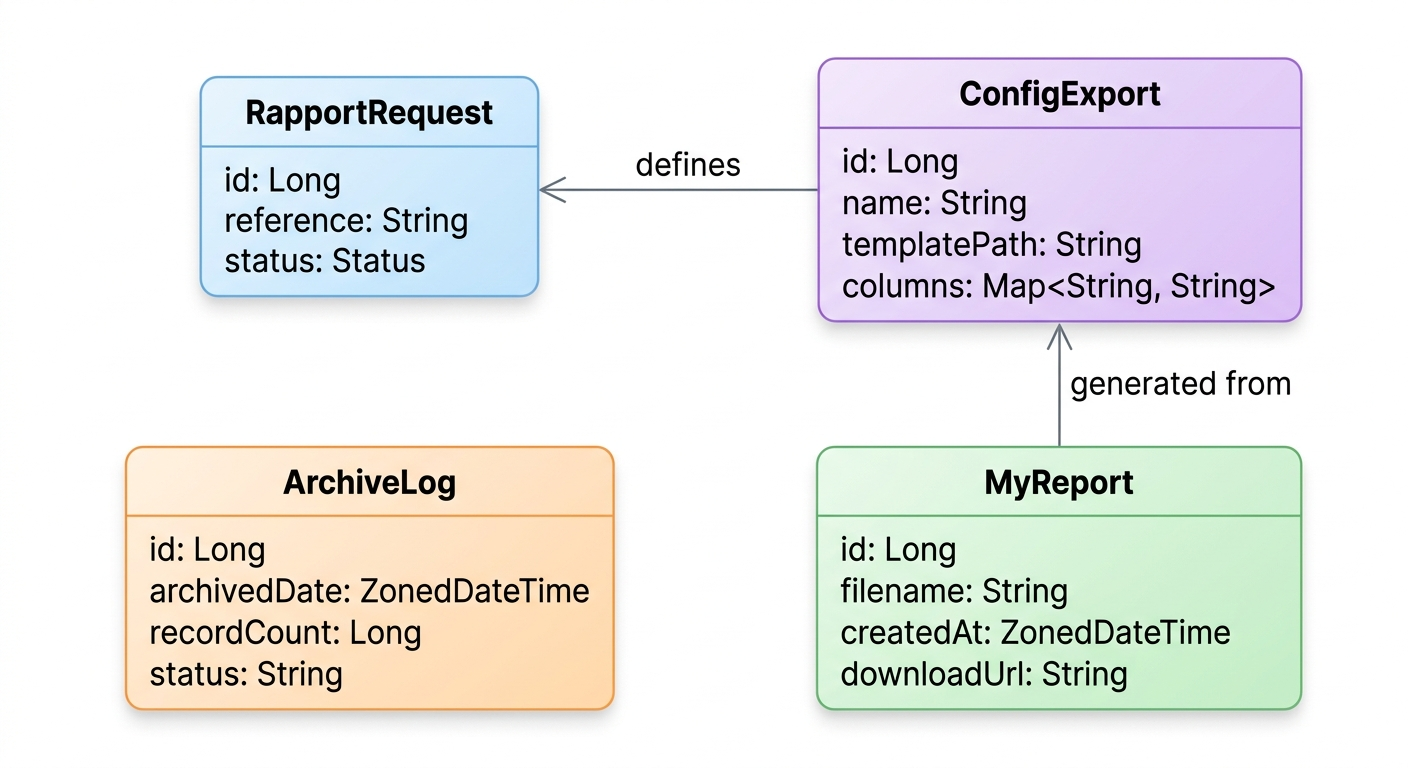
\includegraphics[width=1\textwidth]{class.png}
Class diagram illustrating the Report Manager system
}}
\caption{Sprint 5 Class Diagram}
\label{fig:sprint5_class}
\end{figure}

\section{Realization}

\subsection{Architecture Overview}

Sprint 5 realization focused on two main goals:

\begin{itemize}
\item \textbf{Advanced Reporting:} Enable dynamic Excel report generation based on configurable templates and user-defined filters.
\item \textbf{System Optimization:} Ensure scalability, query efficiency, caching, and automated archival for high-volume intervention data.
\end{itemize}

% The system leverages existing intervention and template domains while adding new services and configurations for reporting and optimization.

\subsection{Backend Implementation Logic}

% Backend services were designed to handle configurable, scalable, and reusable reporting operations:

\begin{itemize}
\item \textbf{ConfigExport Service:} Manages report templates with dynamic column mapping and template activation.
\item \textbf{ExcelReportService:} 
  \begin{itemize}
    \item Queries intervention data based on dynamic filters.
    \item Populates Excel reports using the configured template mapping.
    \item Computes metrics and aggregates without hard-coded field displays.
    \item Handles file creation, storage, and download preparation.
  \end{itemize}
\item \textbf{ArchiveService:} 
  \begin{itemize}
    \item Implements automatic archival of old interventions.
    \item Integrates with external storage solutions for cold data.
    \item A scheduled Maven-based cron job runs every day at 3:00 AM according to project specifications.
    \item It retrieves and processes images of tickets exceeding the days to archive threshold in the \texttt{rapport\_template} table.
    \item It stores archived images in a backup machine, ensuring consistent and reliable data preservation.
  \end{itemize}
\item \textbf{REST Controllers:} Expose endpoints for:
  \begin{itemize}
    \item Dynamic report generation.
    \item Configurable template CRUD operations.
    \item Filtered intervention retrieval for reporting.
  \end{itemize}
\end{itemize}

\subsection{Performance and Optimization Logic}

\begin{itemize}
\item \textbf{Query Optimization:} JPA specifications and fetch strategies avoid N+1 queries, and support large datasets efficiently.
\item \textbf{Caching:} Frequently accessed data (e.g., report templates, intervention summaries) is cached for faster retrieval.
\item \textbf{Archival Scheduling:} Automated cron jobs archive old interventions and maintain system performance.
\item \textbf{Monitoring Integration:} Tracks key metrics such as database query performance, cache hit rates, memory usage, and request statistics.
\end{itemize}

\subsection{Frontend and Integration Logic}

\begin{itemize}
\item Dynamic Rendering of report generation options based on selected templates.
\item Users select filters and templates without hard-coded column mapping.
\item Report download is handled as a fileStream allowing seamless interaction with large datasets.
\item Archival operations are invisible to users but logged for audit purposes.
\end{itemize}

\begin{figure}[H]
\centering
\fbox{\parbox{1\textwidth}{
\centering
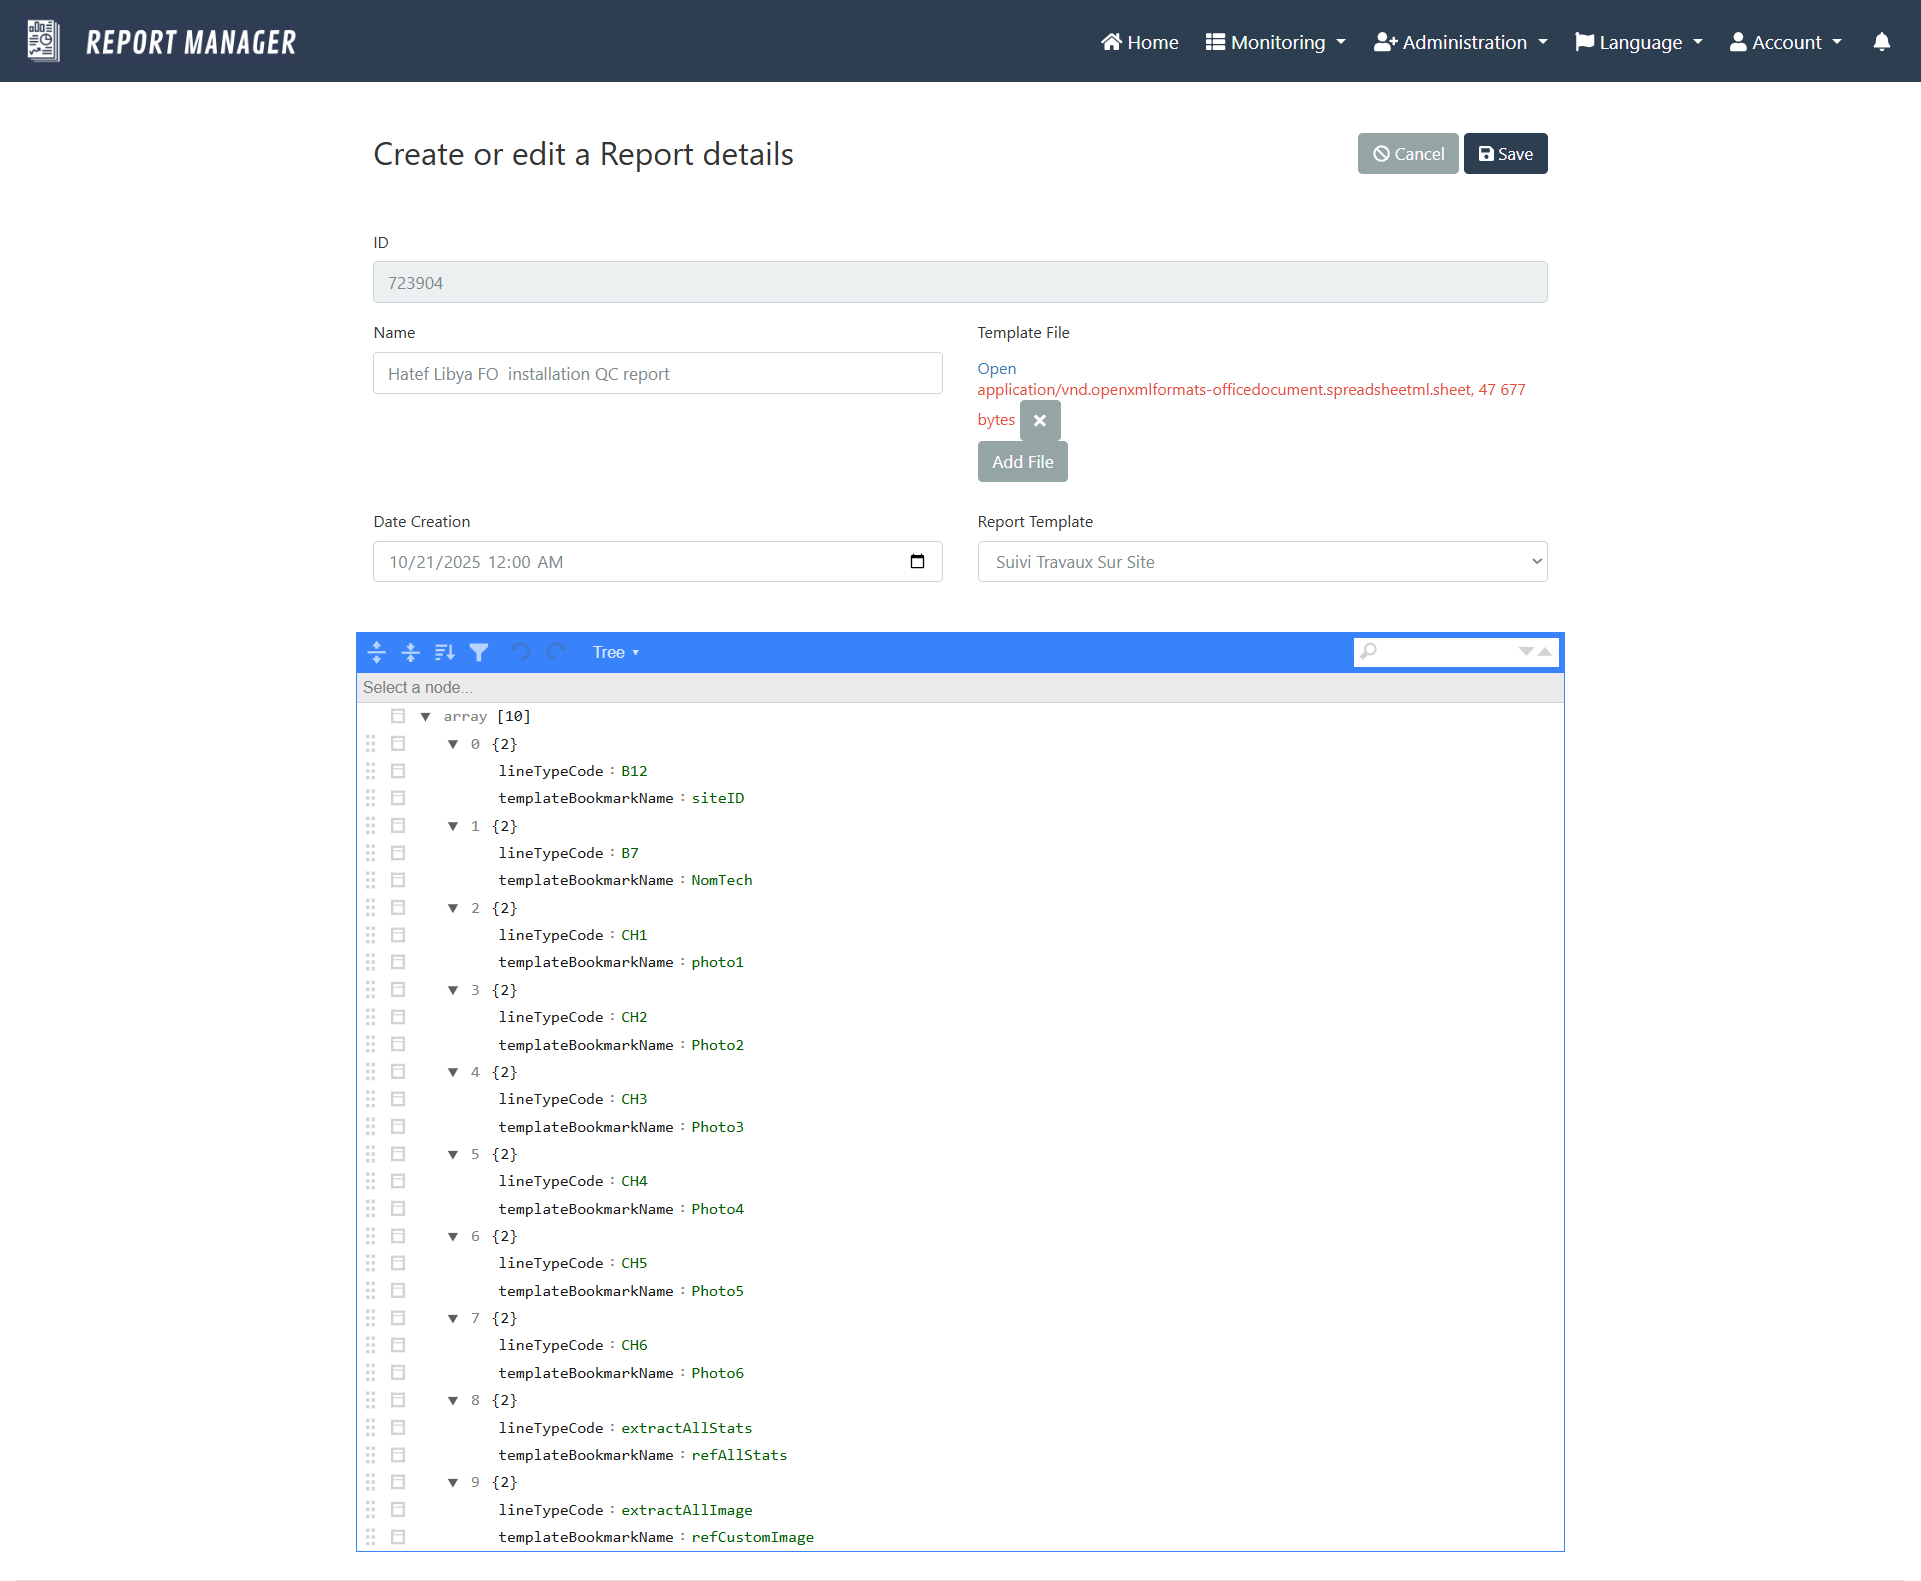
\includegraphics[width=1\textwidth]{outputDef.png}
Example of a configurable Excel report template with dynamic column mapping
}}
\caption{Sprint 5 Output Definition}
\label{fig:sprint5_output}
\end{figure}

\begin{figure}[H]
\centering
\fbox{\parbox{1\textwidth}{
\centering
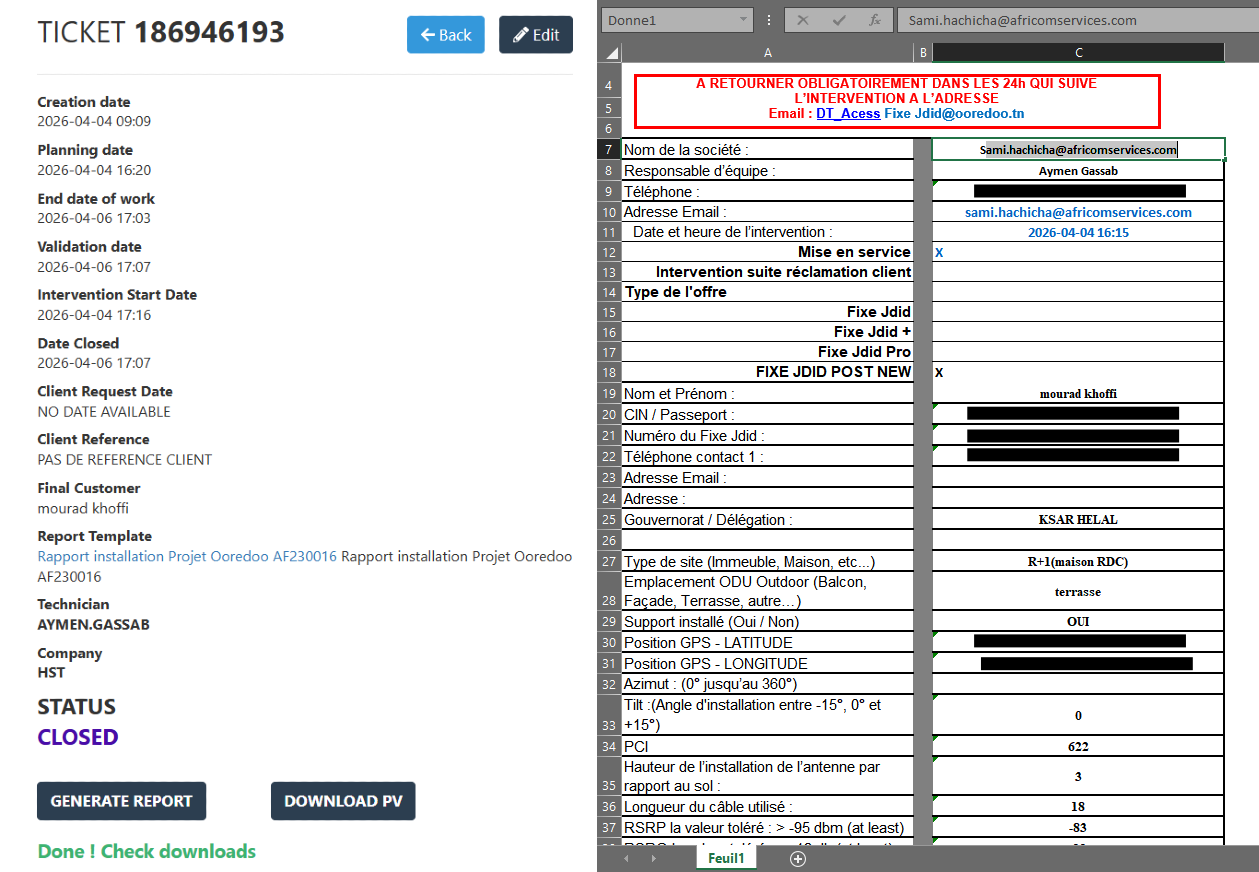
\includegraphics[width=1\textwidth]{gen.png}
Example of a dynamically generated Excel report based on intervention data
}}
\caption{Sprint 5 Generated Report}
\label{fig:sprint5_generated}
\end{figure}


\begin{figure}[H]
\centering
\fbox{\parbox{1\textwidth}{
\centering
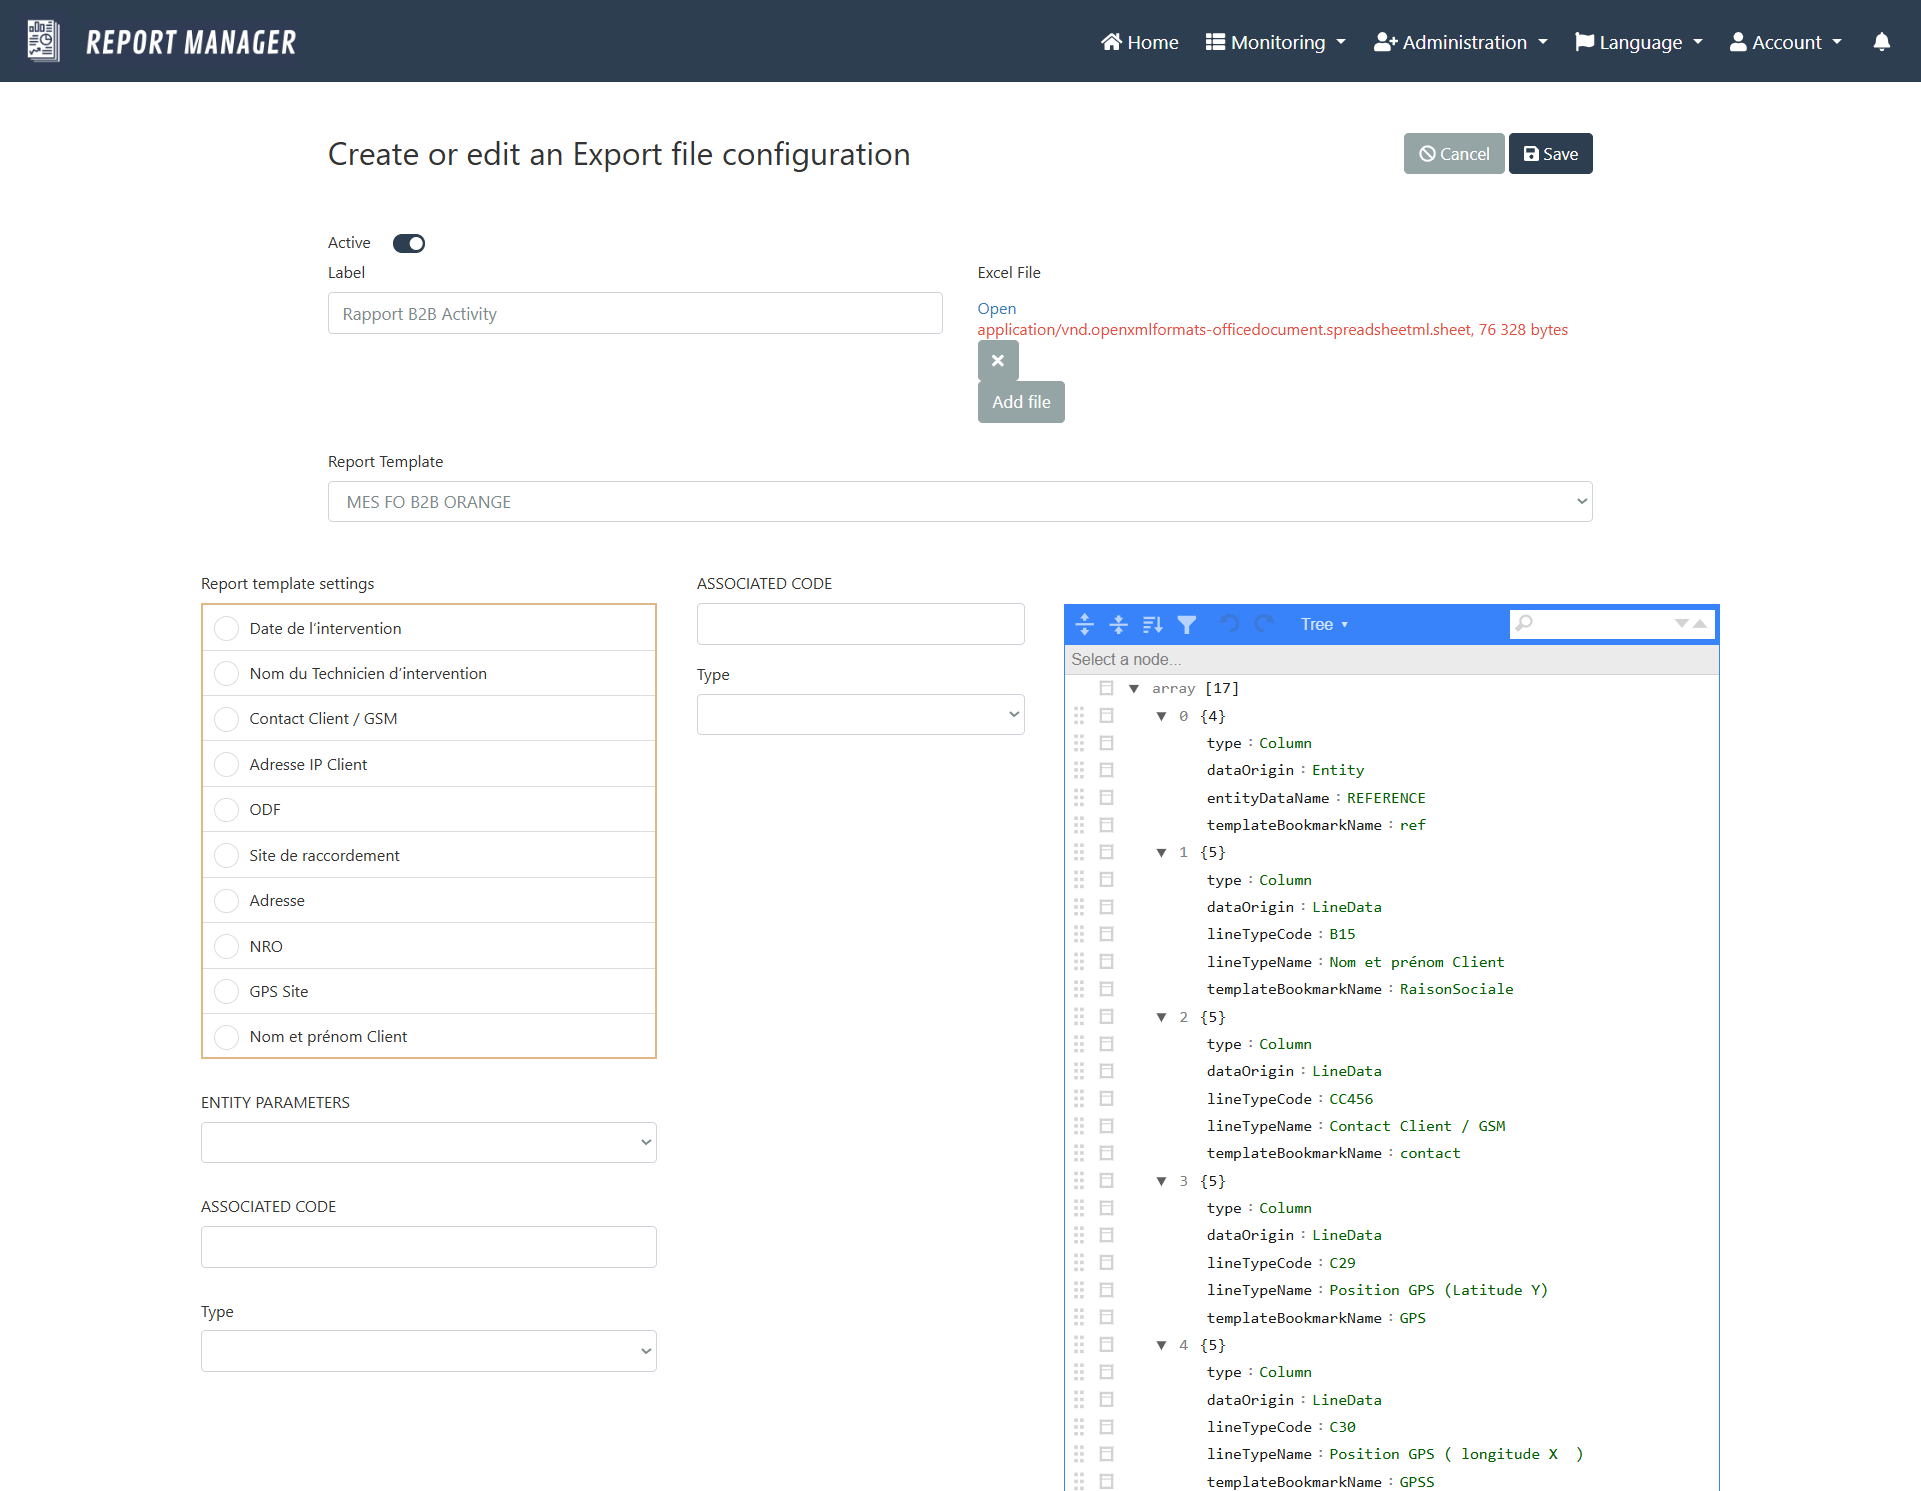
\includegraphics[width=1\textwidth]{conf1.png}
Example of a configurable Excel activity report template with dynamic column mapping
}}
\caption{Sprint 5 Configurable Template}
\label{fig:sprint5_configurable}
\end{figure}


\begin{figure}[H]
\centering
\fbox{\parbox{1\textwidth}{
\centering
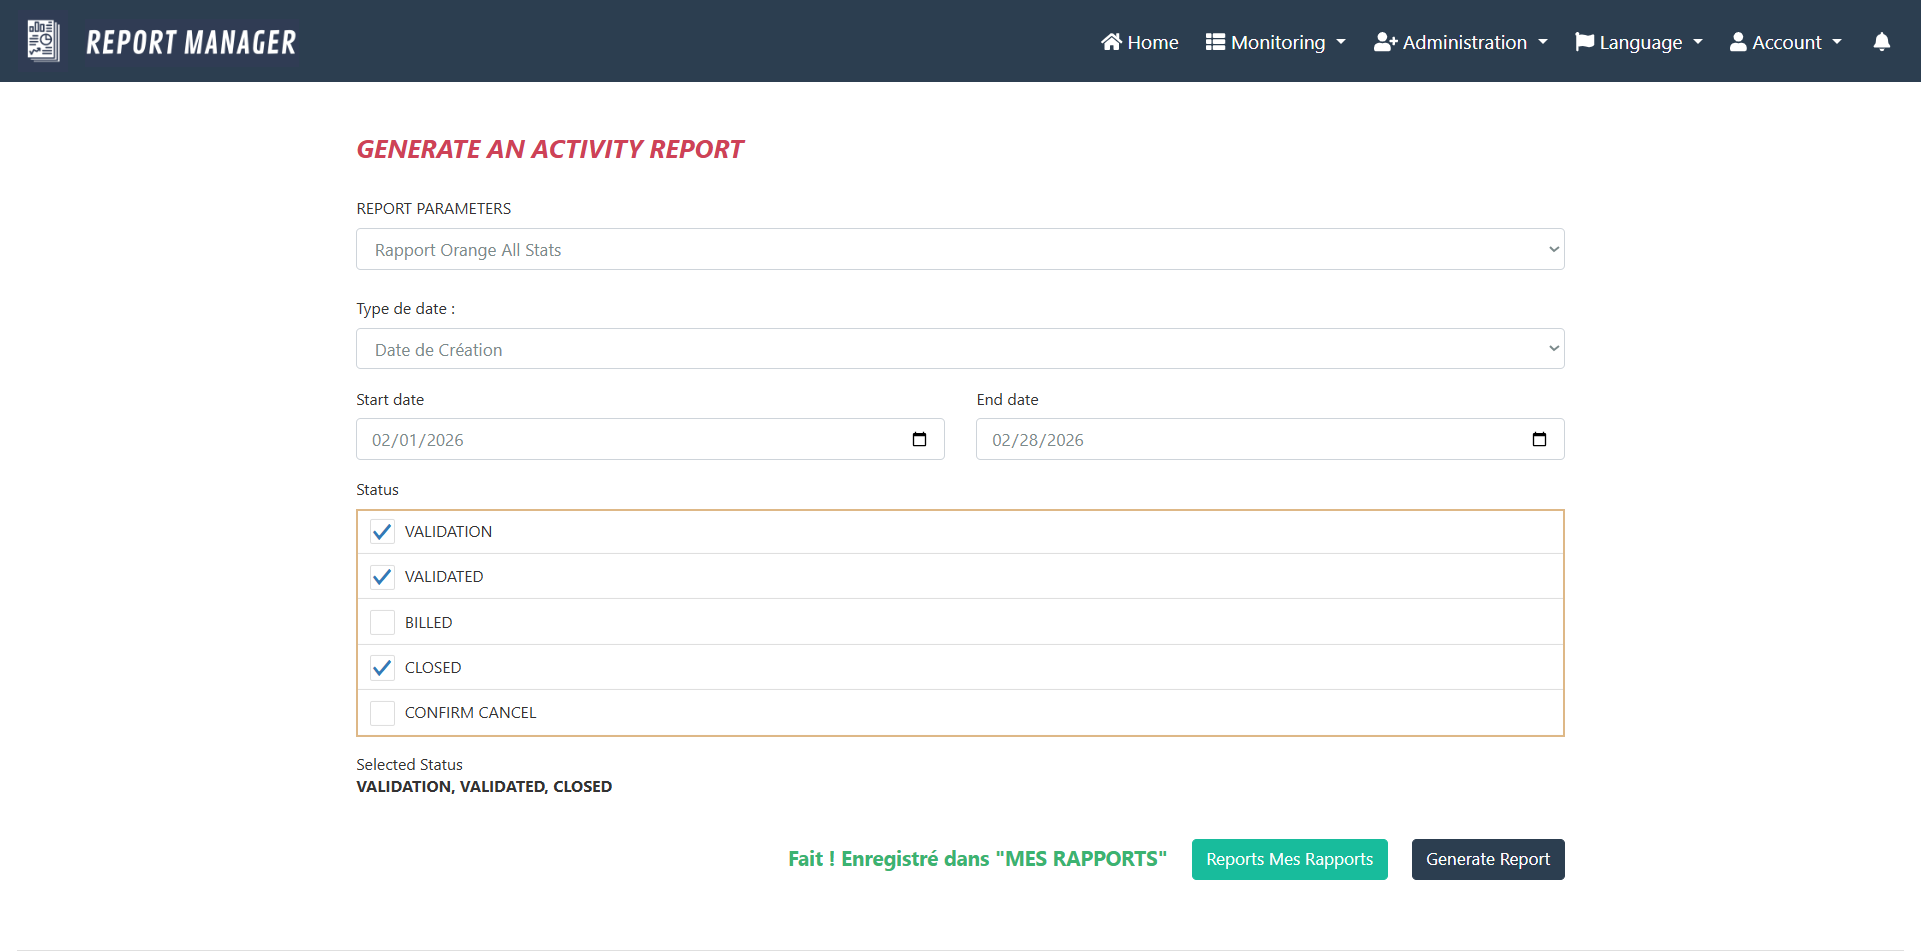
\includegraphics[width=1\textwidth]{conf2.png}
File configuration for a custom Excel report template with dynamic column mapping
}}
\caption{Sprint 5 File Configuration}
\label{fig:sprint5_file_config}
\end{figure}


\begin{figure}[H]
\centering
\fbox{\parbox{1\textwidth}{
\centering
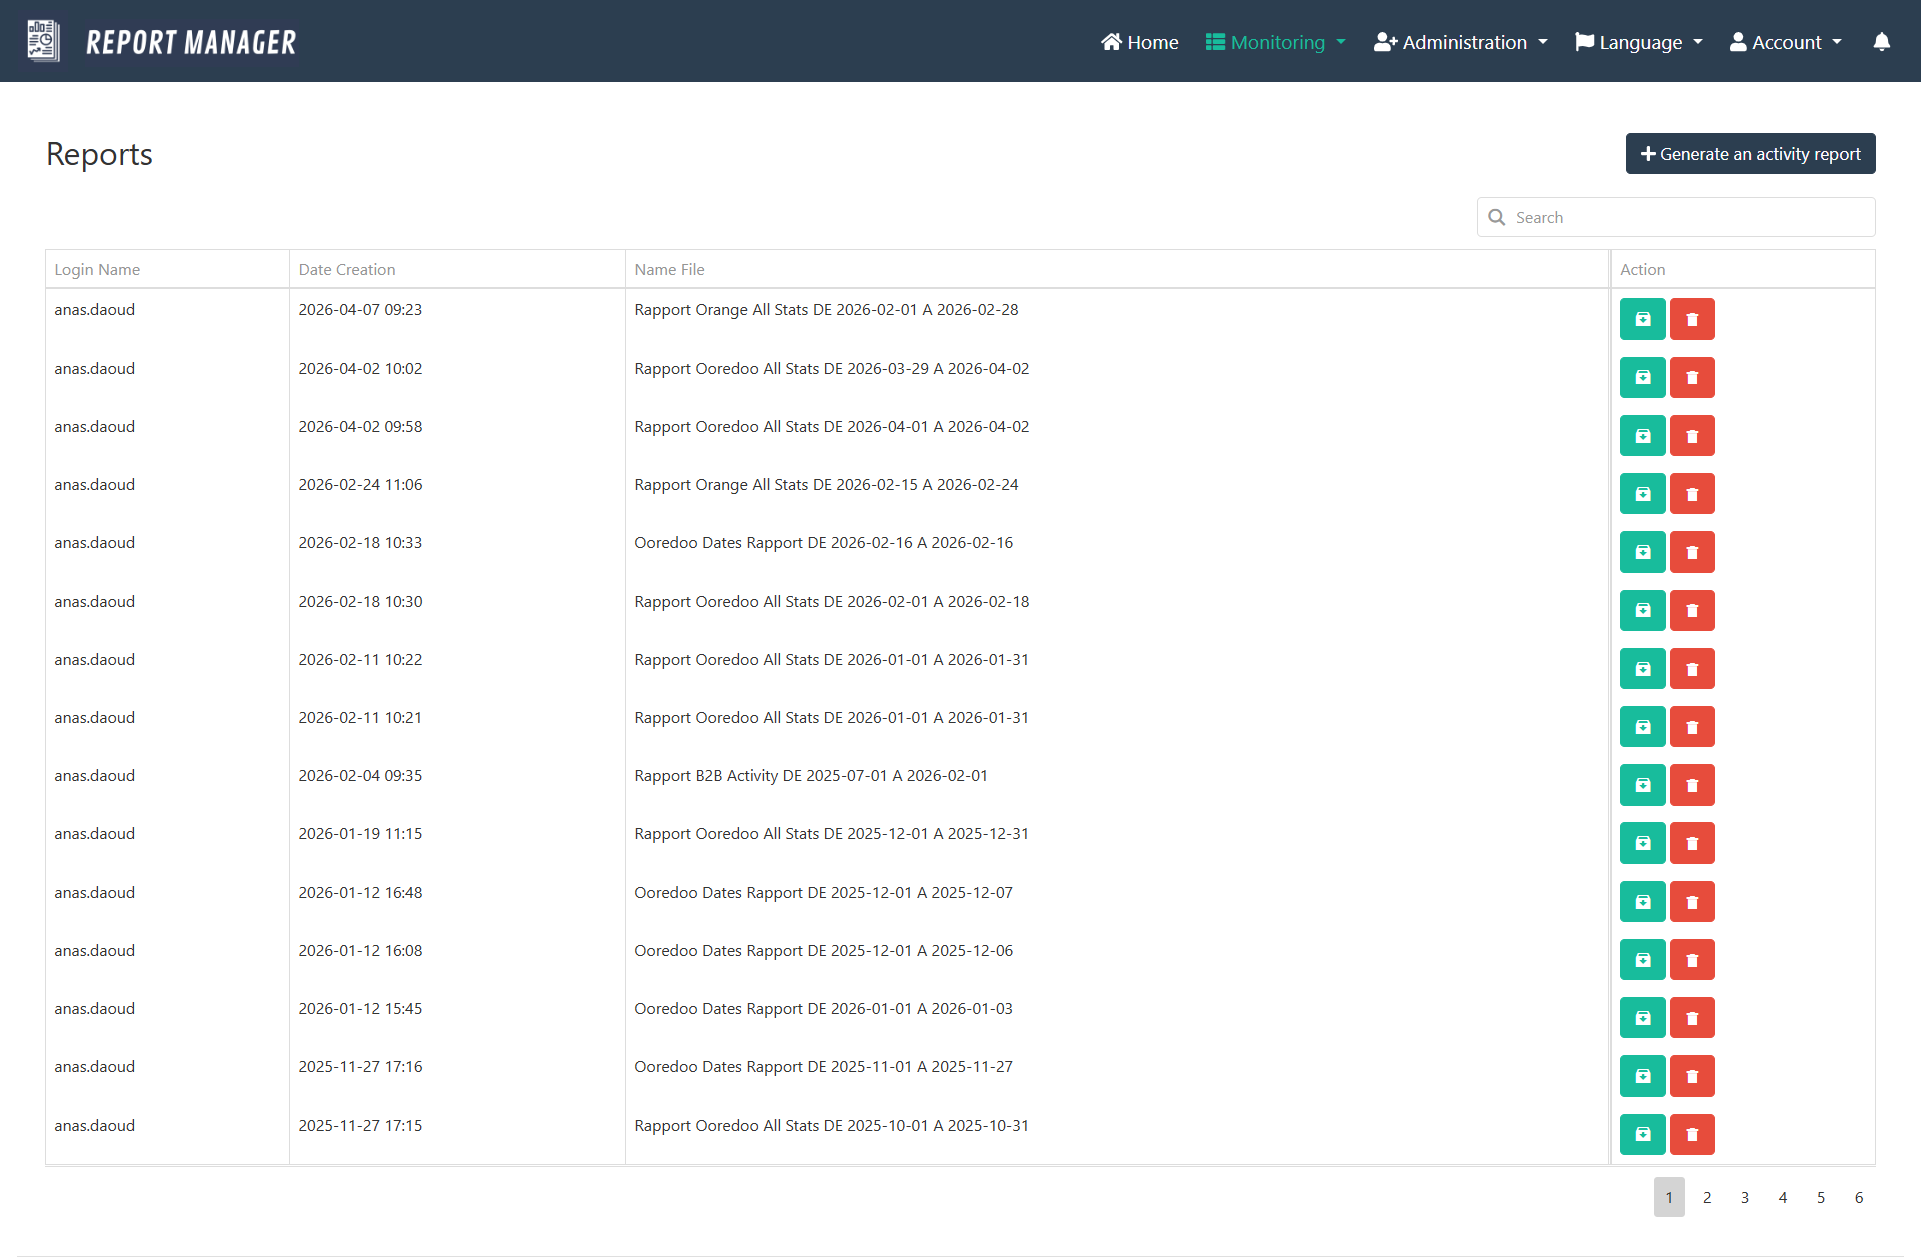
\includegraphics[width=1\textwidth]{conf3.png}
List of Generated Activity Report Excel Files with timestamps and download links
}}
\caption{Sprint 5 List of Generated Reports Links}
\label{fig:sprint5_generated}
\end{figure}


\begin{figure}[H]
\centering
\fbox{\parbox{1\textwidth}{
\centering
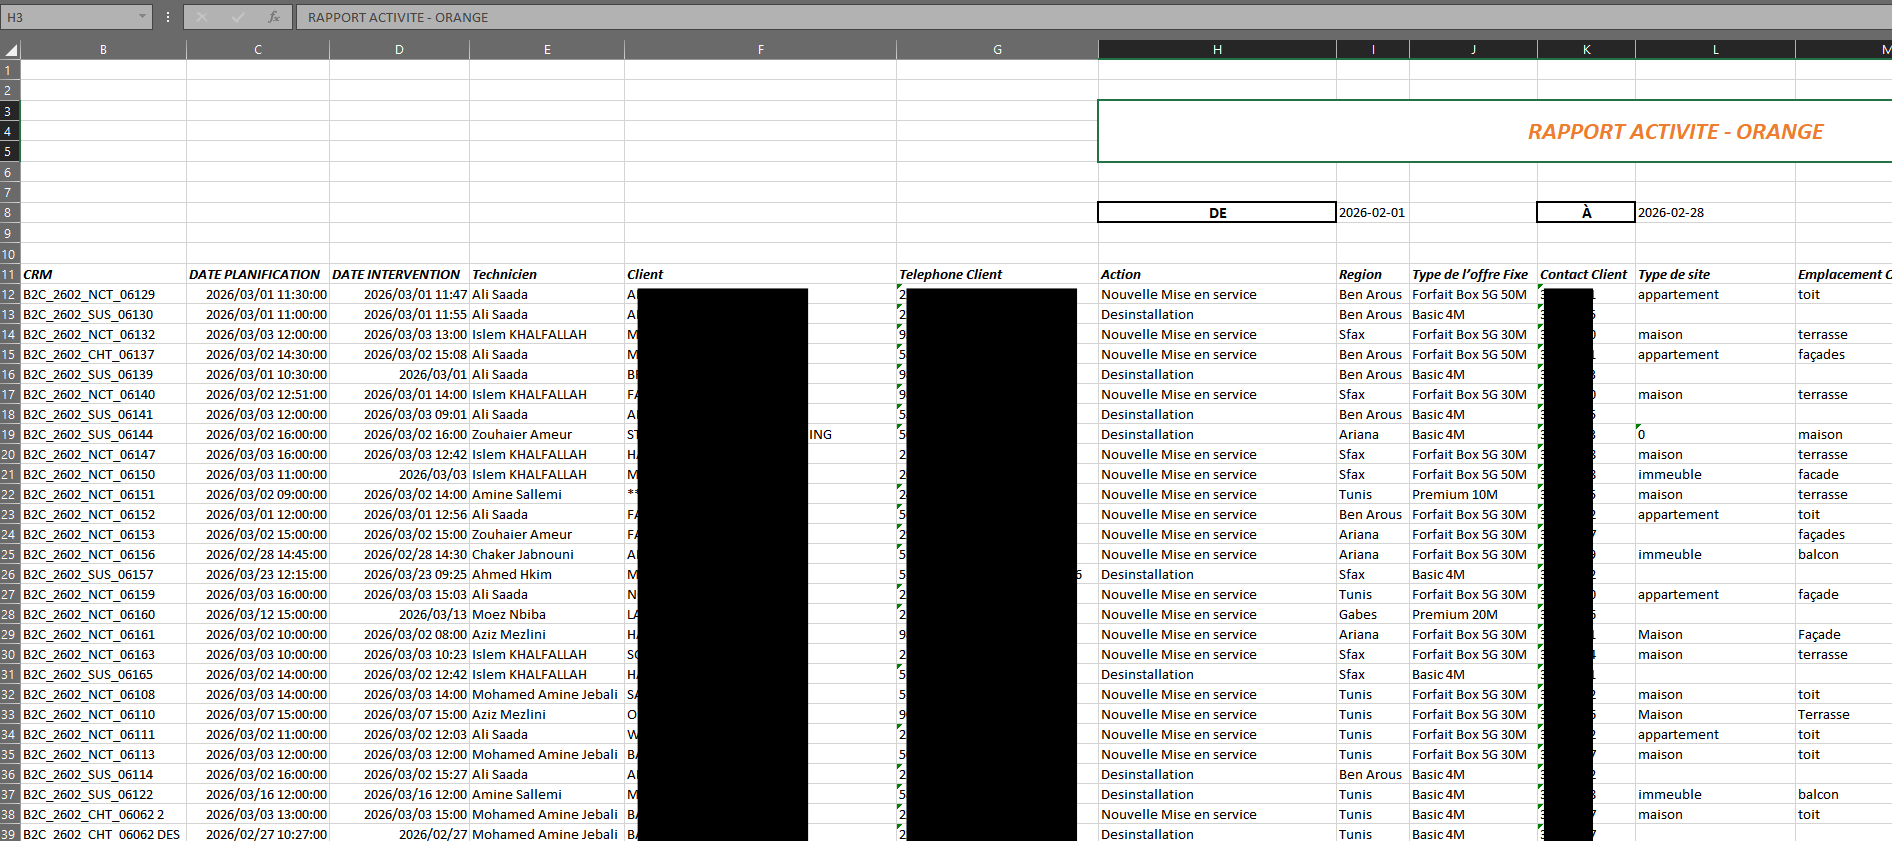
\includegraphics[width=1\textwidth]{conf4.png}
Example of a generated Excel report with dynamic data population and formatting
}}
\caption{Sprint 5 Generated Report}
\label{fig:sprint5_generated}
\end{figure}

\subsection{Key Achievements}

\begin{itemize}
\item Dynamic and reusable Excel reporting system.
\item Template-based column configuration to align with organizational standards.
\item Efficient data retrieval and aggregation for high-volume intervention records.
\item Automated archival process maintaining database performance.
\item System monitoring enabling proactive detection of performance bottlenecks.
\end{itemize}
\section{System Metrics and Monitoring}

The system includes comprehensive monitoring integration:

\begin{table}[H]
\centering
\caption{Key Monitored Metrics}
\label{tab:metrics}
\begin{tabularx}{\textwidth}{|l|X|}
\hline
\textbf{Metric} & \textbf{Description} \\
\hline
HTTP Requests & Total requests, response times by endpoint \\
\hline
Database Queries & Query count, slow query detection \\
\hline
Cache Hit Rate & Cache effectiveness metrics \\
\hline
Disk Space & File storage and backup monitoring \\
\hline
Memory Usage & Heap usage, garbage collection metrics \\
\hline
Failed Requests & Error rates and error type distribution \\
\hline
\end{tabularx}
\end{table}

\begin{figure}[H]
\centering
\fbox{\parbox{1\textwidth}{
\centering
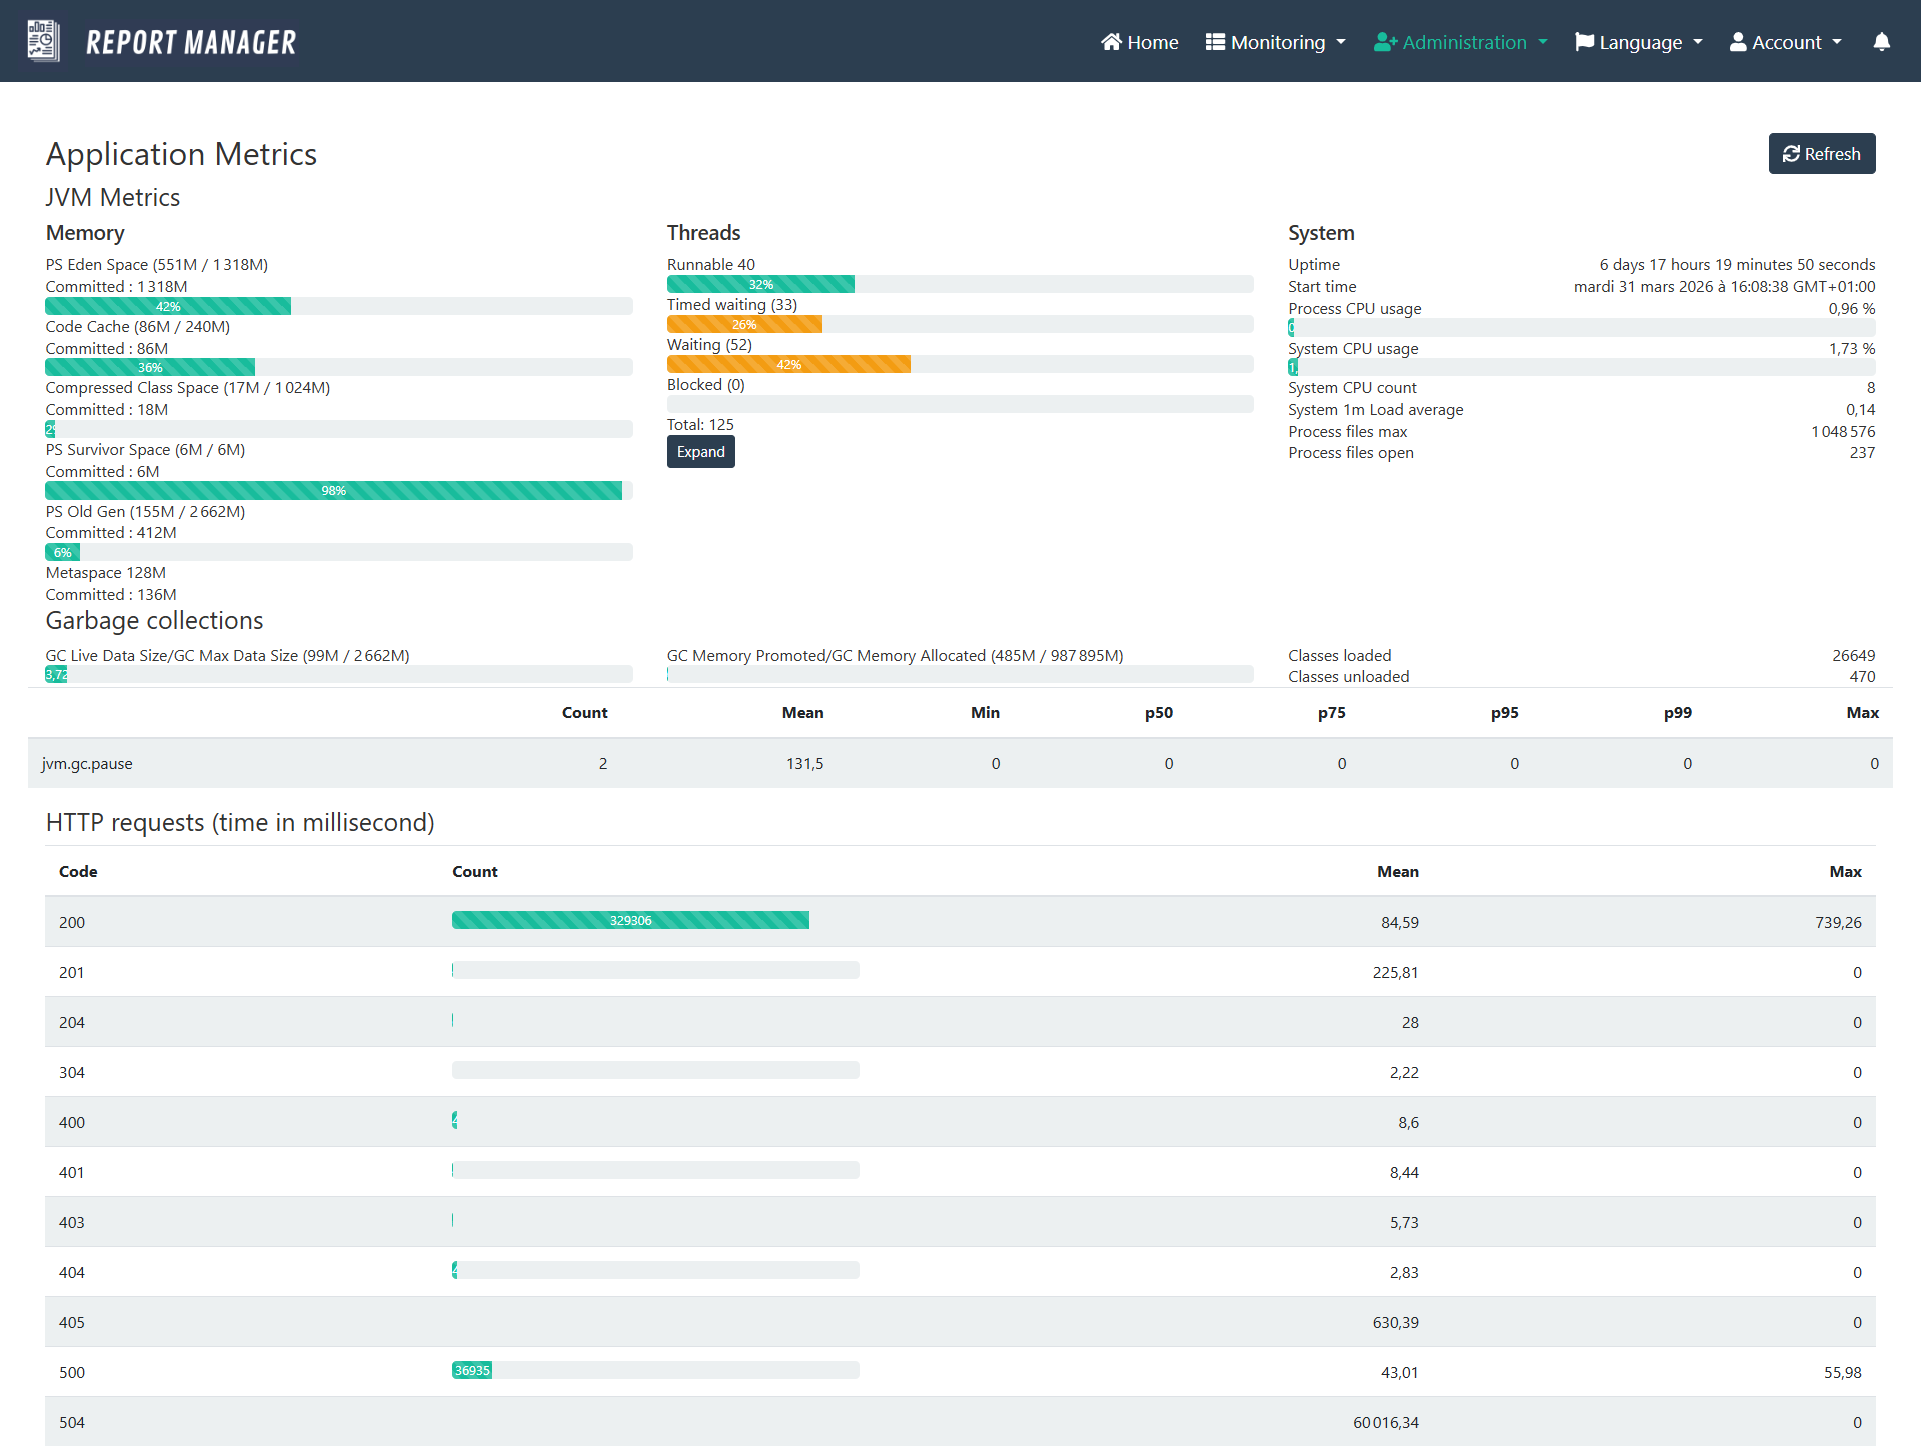
\includegraphics[width=1\textwidth]{mzt.png}
System monitoring dashboard illustrating key performance metrics
}}
\caption{Sprint 5 Monitoring Dashboard}
\label{fig:sprint5_monitoring}
\end{figure}

\section{Conclusion}

Sprint 5 successfully completed the development of the Report Manager system with comprehensive reporting capabilities and production-ready optimization. The Excel report generation enables organizational decision-making and data analysis. Performance optimization ensures the system scales effectively with growing data volumes.

Key achievements:
\begin{itemize}
\item Comprehensive Excel report generation with custom templates
\item Configurable report templates for organizational standards
\item Automated archival strategy for database optimization
\item Query optimization and intelligent caching
\item System monitoring and health metrics
\end{itemize}

The complete system now provides:
\begin{enumerate}
\item \textbf{Foundation Phase:} Authentication, database, API infrastructure
\item \textbf{Core Functionality:} Intervention management and form templates
\item \textbf{Evidence Management:} File uploads and geolocation tracking
\item \textbf{Quality Assurance:} Approval workflows and status management
\item \textbf{Business Analytics:} Advanced reporting and system optimization
\end{enumerate}

All five development sprints have been successfully completed, delivering a fully functional, production-ready intervention management system.
